
\begin{frame}
\frametitle{University College London}
\begin{tabular}{lcr}
\begin{minipage}[l]{5.0cm}
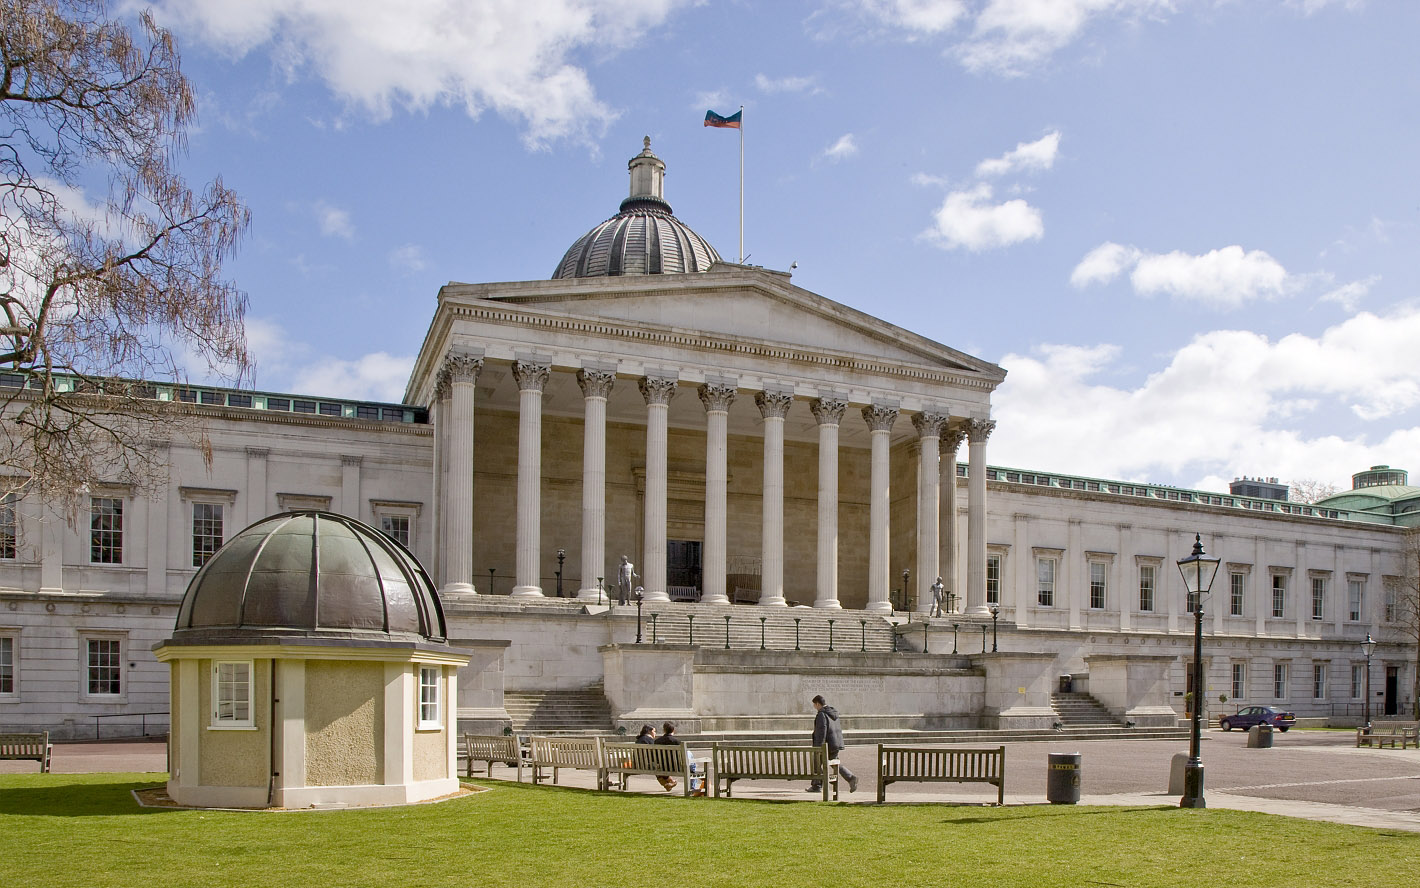
\includegraphics[height=3.8cm]{ucl_building}
\end{minipage} & &
\begin{minipage}[r]{6.5cm}
\begin{itemize}
\item UCL was rated 2nd in the UK for research power in the Research Excellence Framework 2021
\item UCL is ranked 8th in the 2022 QS World University Rankings
\item The Department of Statistical Science has played a major role in the development of the subject ever since its foundation in 1911 as the Department of Applied Statistics
\end{itemize}
\end{minipage}
\end{tabular}
\end{frame}

\begin{frame}%[noframenumbering]
\frametitle{Objective of this course}

\only<1>{
\begin{tabular}{lcr}
\begin{minipage}[l]{5.0cm}
\textbf{Lectures}\\
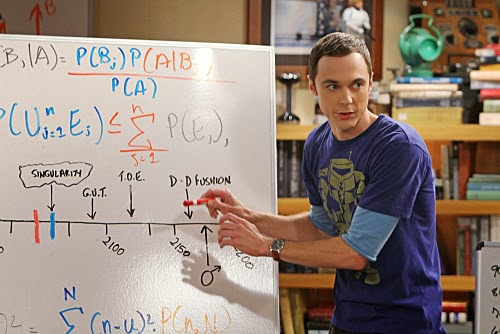
\includegraphics[height=3.8cm]{Lecture}
\end{minipage} & &
\begin{minipage}[r]{6.5cm}
\begin{itemize}
\item Introduction to \alert{Health economic evaluation}
\begin{itemize}
\item ICER, EIB
\item Cost-effectiveness plane, CEAC
\end{itemize}
\vspace{10pt}
\item Introduction to \alert{Bayesian analysis}
\begin{itemize}
\item MCMC methods
\item Using \texttt{BUGS} (and \texttt{R})
\end{itemize}
\vspace{10pt}
\item Introduction to \alert{Health economics modelling}
\begin{itemize}
\item Decision trees
\item Markov models
\end{itemize}
\end{itemize}
\end{minipage}
\end{tabular}}

\only<2>{
\begin{tabular}{lcr}
\begin{minipage}[l]{5.0cm}
\textbf{Computer practicals}\\
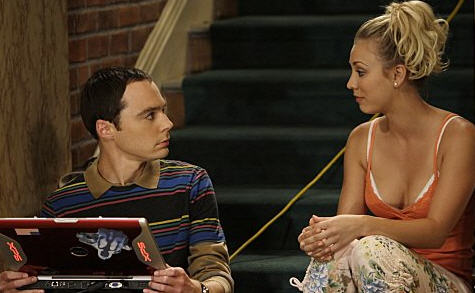
\includegraphics[height=3.5cm]{Practical}
\end{minipage} & &
\begin{minipage}[r]{6.5cm}
\begin{itemize}
\item Emphasis on practical examples
\begin{itemize}
\item \texttt{BUGS} analysis
\item \texttt{R}/\texttt{BUGS} and \texttt{BCEA}
\end{itemize}
\end{itemize}
\end{minipage} 
\end{tabular}}
\end{frame}

\frame{
\frametitle{Timetable}
\begin{itemize}
\item[] \textbf{Day 1}
\begin{itemize}
\item 9:00-9:10 Welcome and introductions
\item 9:10-10:00 Introduction to health economic evaluations
\item 10:00-11:00 Cost and cost-utility data
\item BREAK
\item 11:30-12:30 Model error and structural uncertainty
\item LUNCH
\item 1:30-2:30 Decision trees in HEE
\item 2:30-3:30 Markov models in HEE
\item BREAK
\item 4:00-5:00 Review and wrap up
\end{itemize}

\vspace{5pt}\pause
\item[] \textbf{Day 2}
\begin{itemize}
\item Welcome and introductions
\item Building a basic decision tree in R
\item Building more complex tree in R
\item BREAK
\item 11:30-12:30 Building a simple Markov model in R
\item LUNCH
\item 1:30-2:30 Building a more complex Markov model in R
\item 2:30-3:30 Sensitivity analysis
\item BREAK
\item 4:00-5:00 Visualising cost-effectiveness analyses with the BCEA package
\item 5:00 Wrap up and thanks
\end{itemize}
\end{itemize}
}

\begin{frame}%[noframenumbering]
\frametitle{More Bayesian Health Economics...}

\begin{tabular}{lcr}
\begin{minipage}[l]{5.0cm}
\textbf{Books}\\
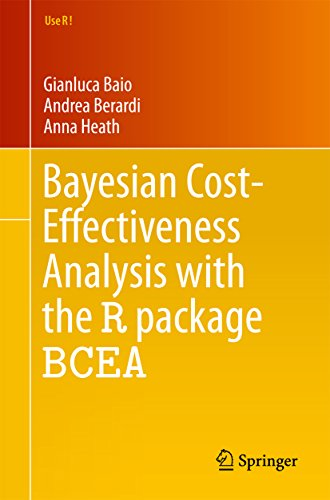
\includegraphics[height=3.8cm]{bcea_book}
\includegraphics[height=3.8cm]{bmhe_book}
\end{minipage} & &
\begin{minipage}[r]{6.5cm}
\begin{itemize}
\item This course is only a small part of an \alert{annual week-long summer school}
\begin{itemize}
\item this year in  UNIL, Université de Lausanne, Lausanne (Switzerland)
\item usually in Florence, Italy
\end{itemize}
\item Several books available
\item Edition two of BCEA book in the pipeline and a Health Economic in R book close to being finished!
\end{itemize}

\end{minipage}
\end{tabular}
\end{frame}

